\documentclass[../Main.tex]{subfiles}
\begin{document}

\section{Methodology: Selective Coordination with Masking}

Our central hypothesis is that enforcing full coordination among all agents at every timestep, as is standard in QMIX, is both computationally inefficient and unnecessary for effective learning. We posit that a more flexible, selective coordination mechanism can reduce complexity while potentially acting as a beneficial regularizer.

\subsection{QMIX-Masked: A Lightweight Architectural Variant}
To test this hypothesis, we propose \textbf{QMIX-Masked}, a variant of QMIX that introduces a dynamic masking mechanism directly before the mixing network, as shown in Figure~\ref{fig:qmix_masked_arch}.

At each timestep \(t\), a binary mask \(M(t) \in \{0,1\}^N\) is generated to determine which agents are "active" in the joint Q-function computation. The masked Q-vector \(\widetilde{\mathbf{q}}(t)\) is then formed by element-wise multiplication:
\[
\widetilde{\mathbf{q}}(t) \;=\; M(t) \odot [\,Q_1(\tau_1,u_1),\,Q_2(\tau_2,u_2),\,\dots,\,Q_N(\tau_N,u_N)\,]
\]
This reduced vector is passed to the mixing network. The state input to the hypernetwork can also be filtered to include information from only the unmasked agents. This approach reduces the effective input size for the centralized components, thereby lowering the computational burden per step.

\begin{figure}[H]
    \centering
    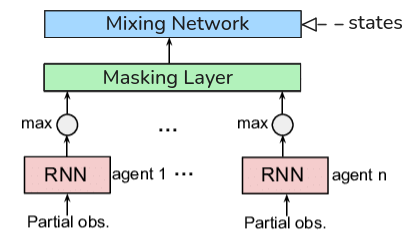
\includegraphics[width=0.7\textwidth]{img/masked-qmix.png}
    \caption{The architecture of QMIX-Masked. A binary mask is applied to the individual agent Q-values before they are fed into the mixing network.}
    \label{fig:qmix_masked_arch}
\end{figure}

\section{Experimental Protocol and Results}

Our investigation into QMIX-Masked follows a structured protocol designed to isolate the effects of masking and rigorously evaluate its impact on performance and robustness.

\subsection{Scenario Selection and Baseline Establishment}
To meaningfully evaluate the performance degradation introduced by masking, we first needed to identify a benchmark scenario where the baseline algorithm, vanilla QMIX, achieves strong and reliable performance. Running experiments on maps where the baseline already fails would make it impossible to distinguish performance loss due to masking from the inherent difficulty of the task.

As shown in Figure~\ref{fig:hard_scenarios_results}, our initial runs confirmed that vanilla QMIX performs poorly on several of the more difficult SMAC scenarios, such as \texttt{6h\_vs\_8z} and \texttt{corridor}. As expected, a preliminary sanity check of QMIX-Masked on these maps also yielded poor results. These scenarios are therefore unsuitable for our primary analysis.


\begin{figure}[H]
    \centering
    % --- ROW 1: TWO COLUMNS ---
    \begin{subfigure}[b]{0.48\textwidth}
        \centering
        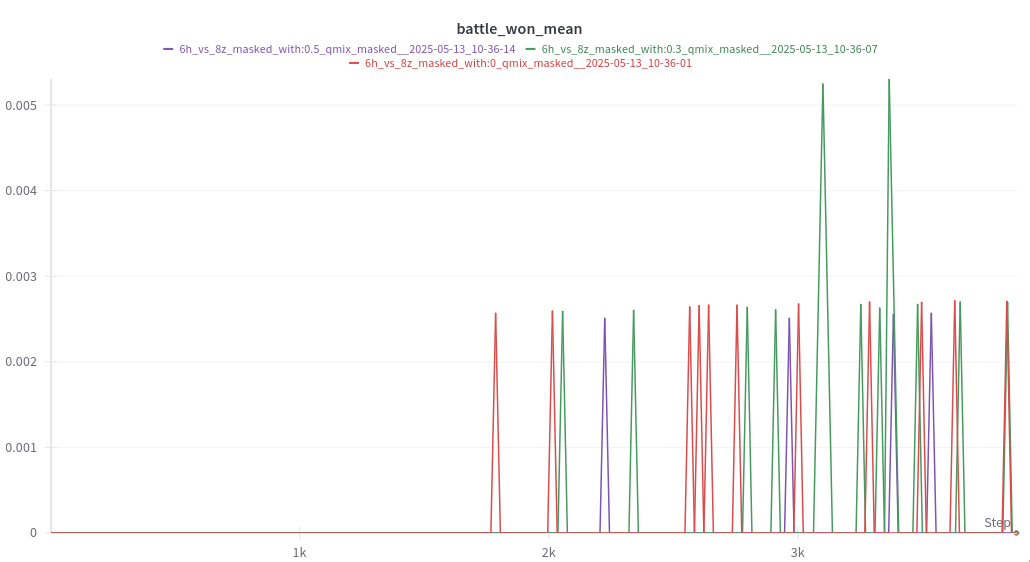
\includegraphics[width=\linewidth]{img/results/6hvs8z.png}
        \caption{\texttt{6h\_vs\_8z} scenario.}
        \label{fig:6hvs8z}
    \end{subfigure}
    \hfill % Pushes the subfigures apart to fill the line
    \begin{subfigure}[b]{0.48\textwidth}
        \centering
        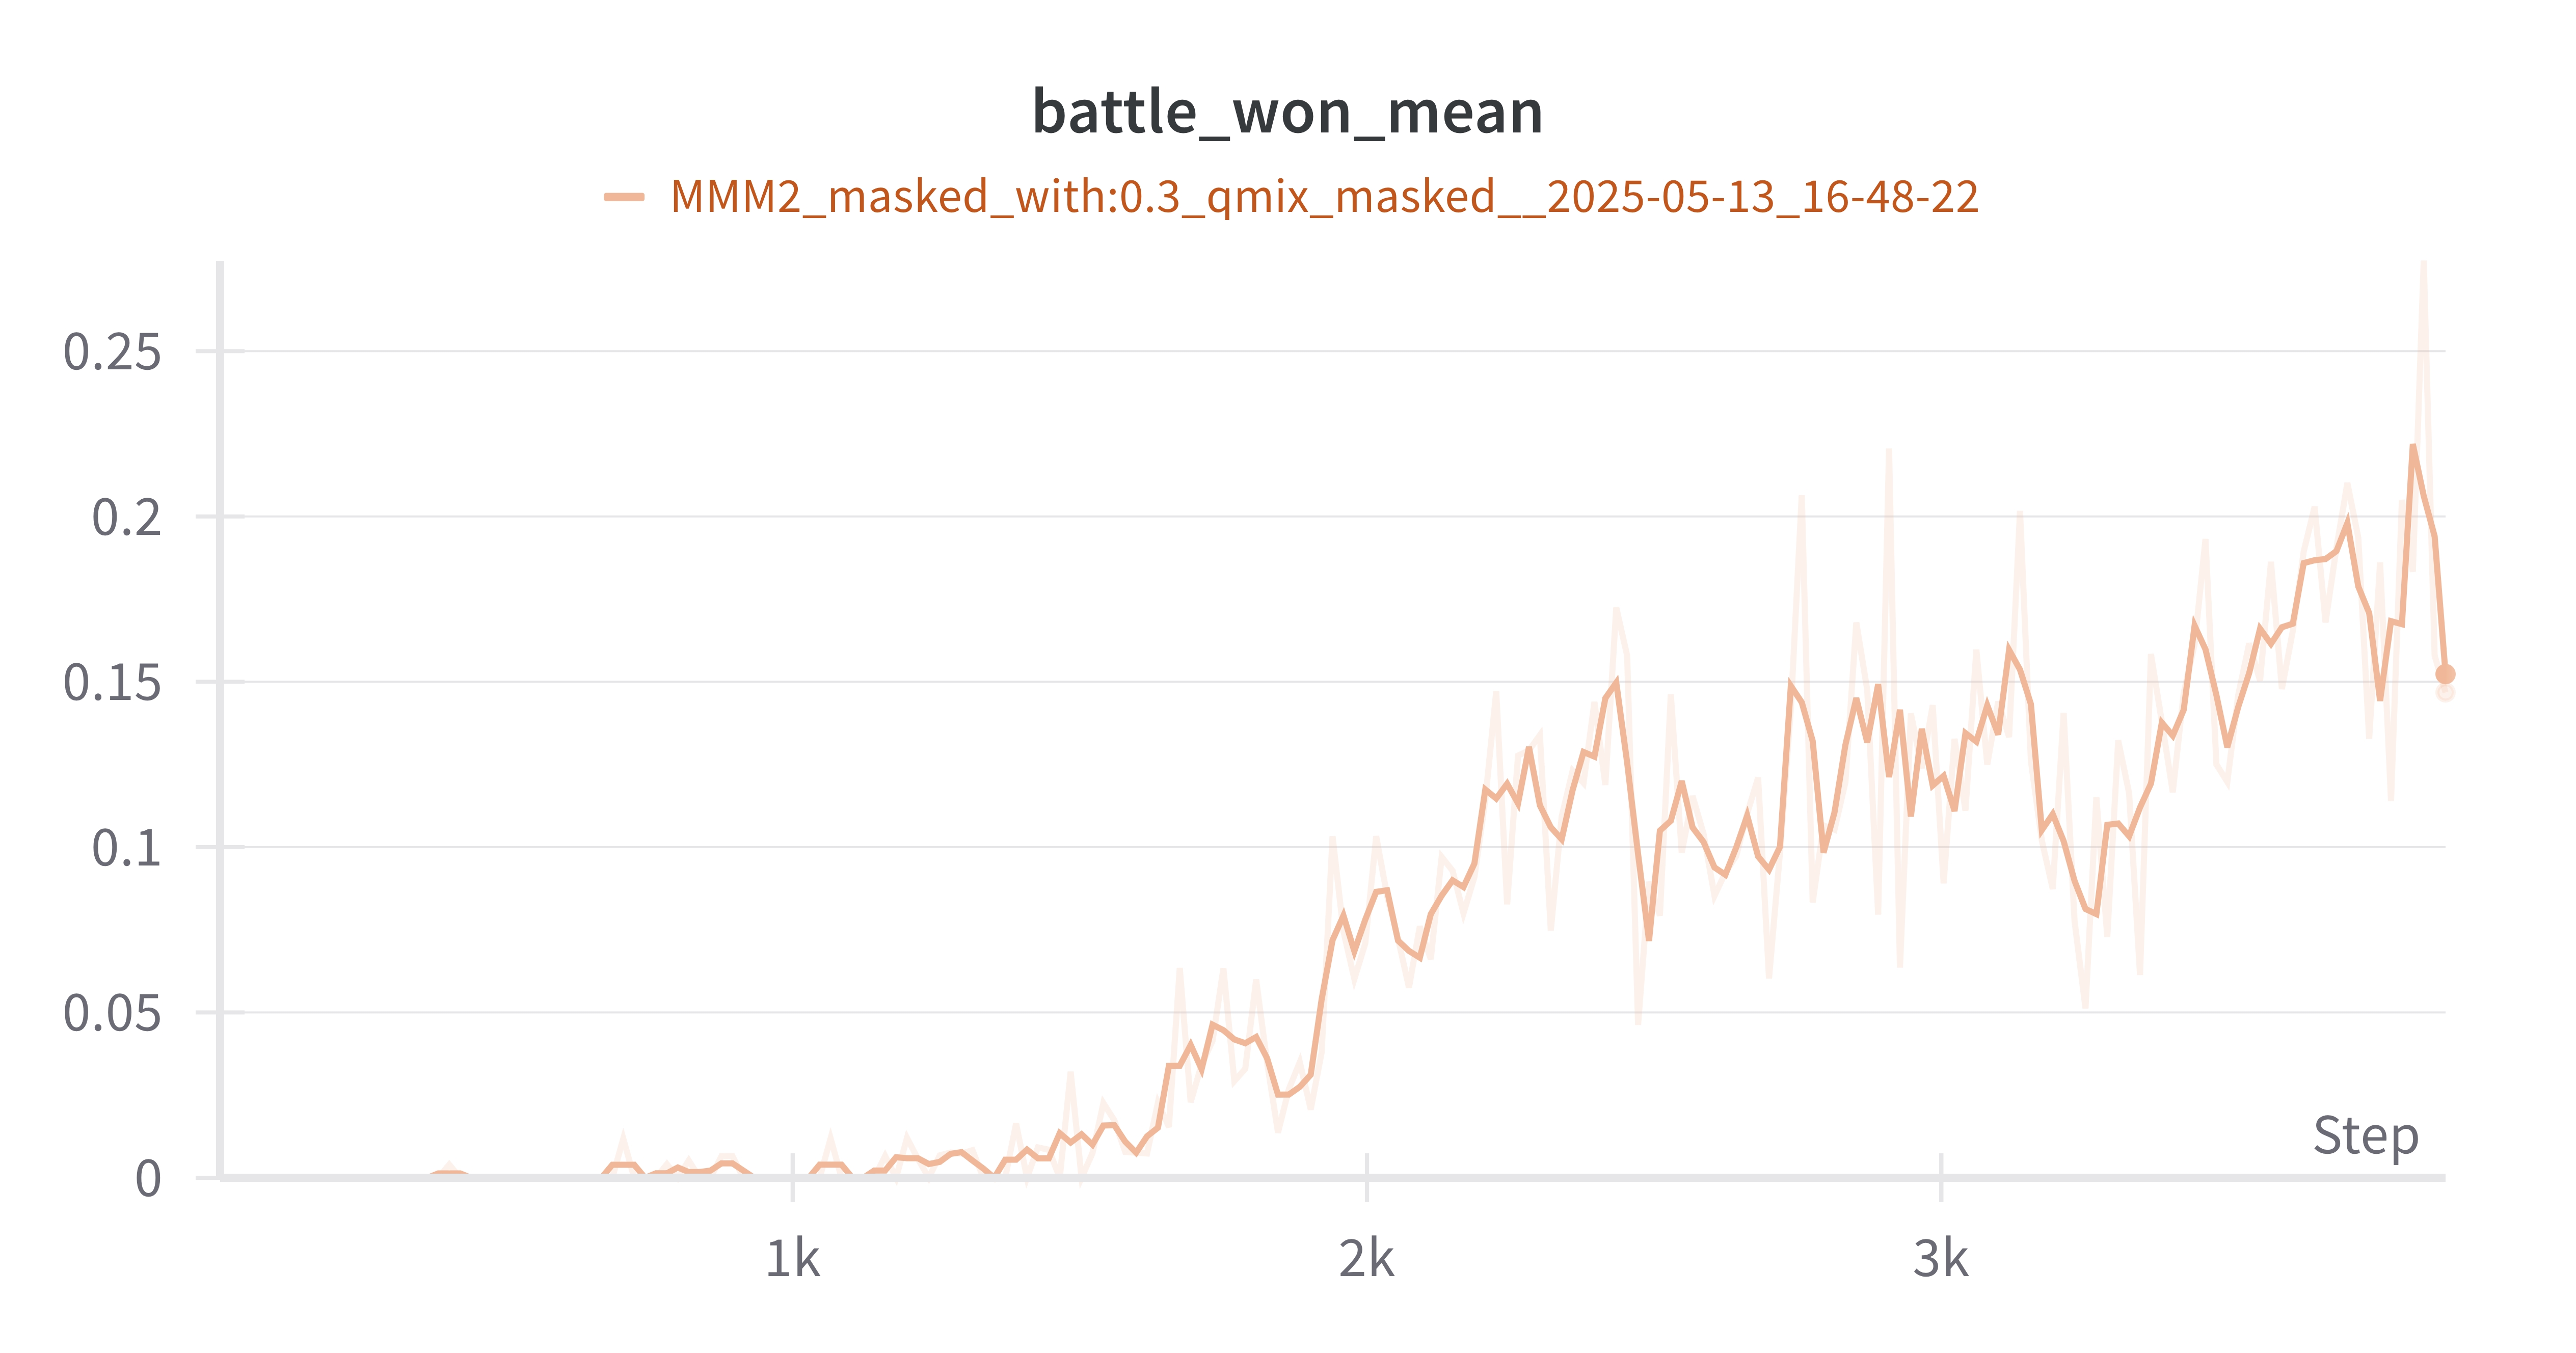
\includegraphics[width=\linewidth]{img/results/MMM2.png}
        \caption{\texttt{MMM2} scenario.}
        \label{fig:mmm2}
    \end{subfigure}
    \vspace{1em} % Adds a bit of vertical space between the rows

    % --- ROW 2: TWO COLUMNS ---
    \begin{subfigure}[b]{0.48\textwidth}
        \centering
        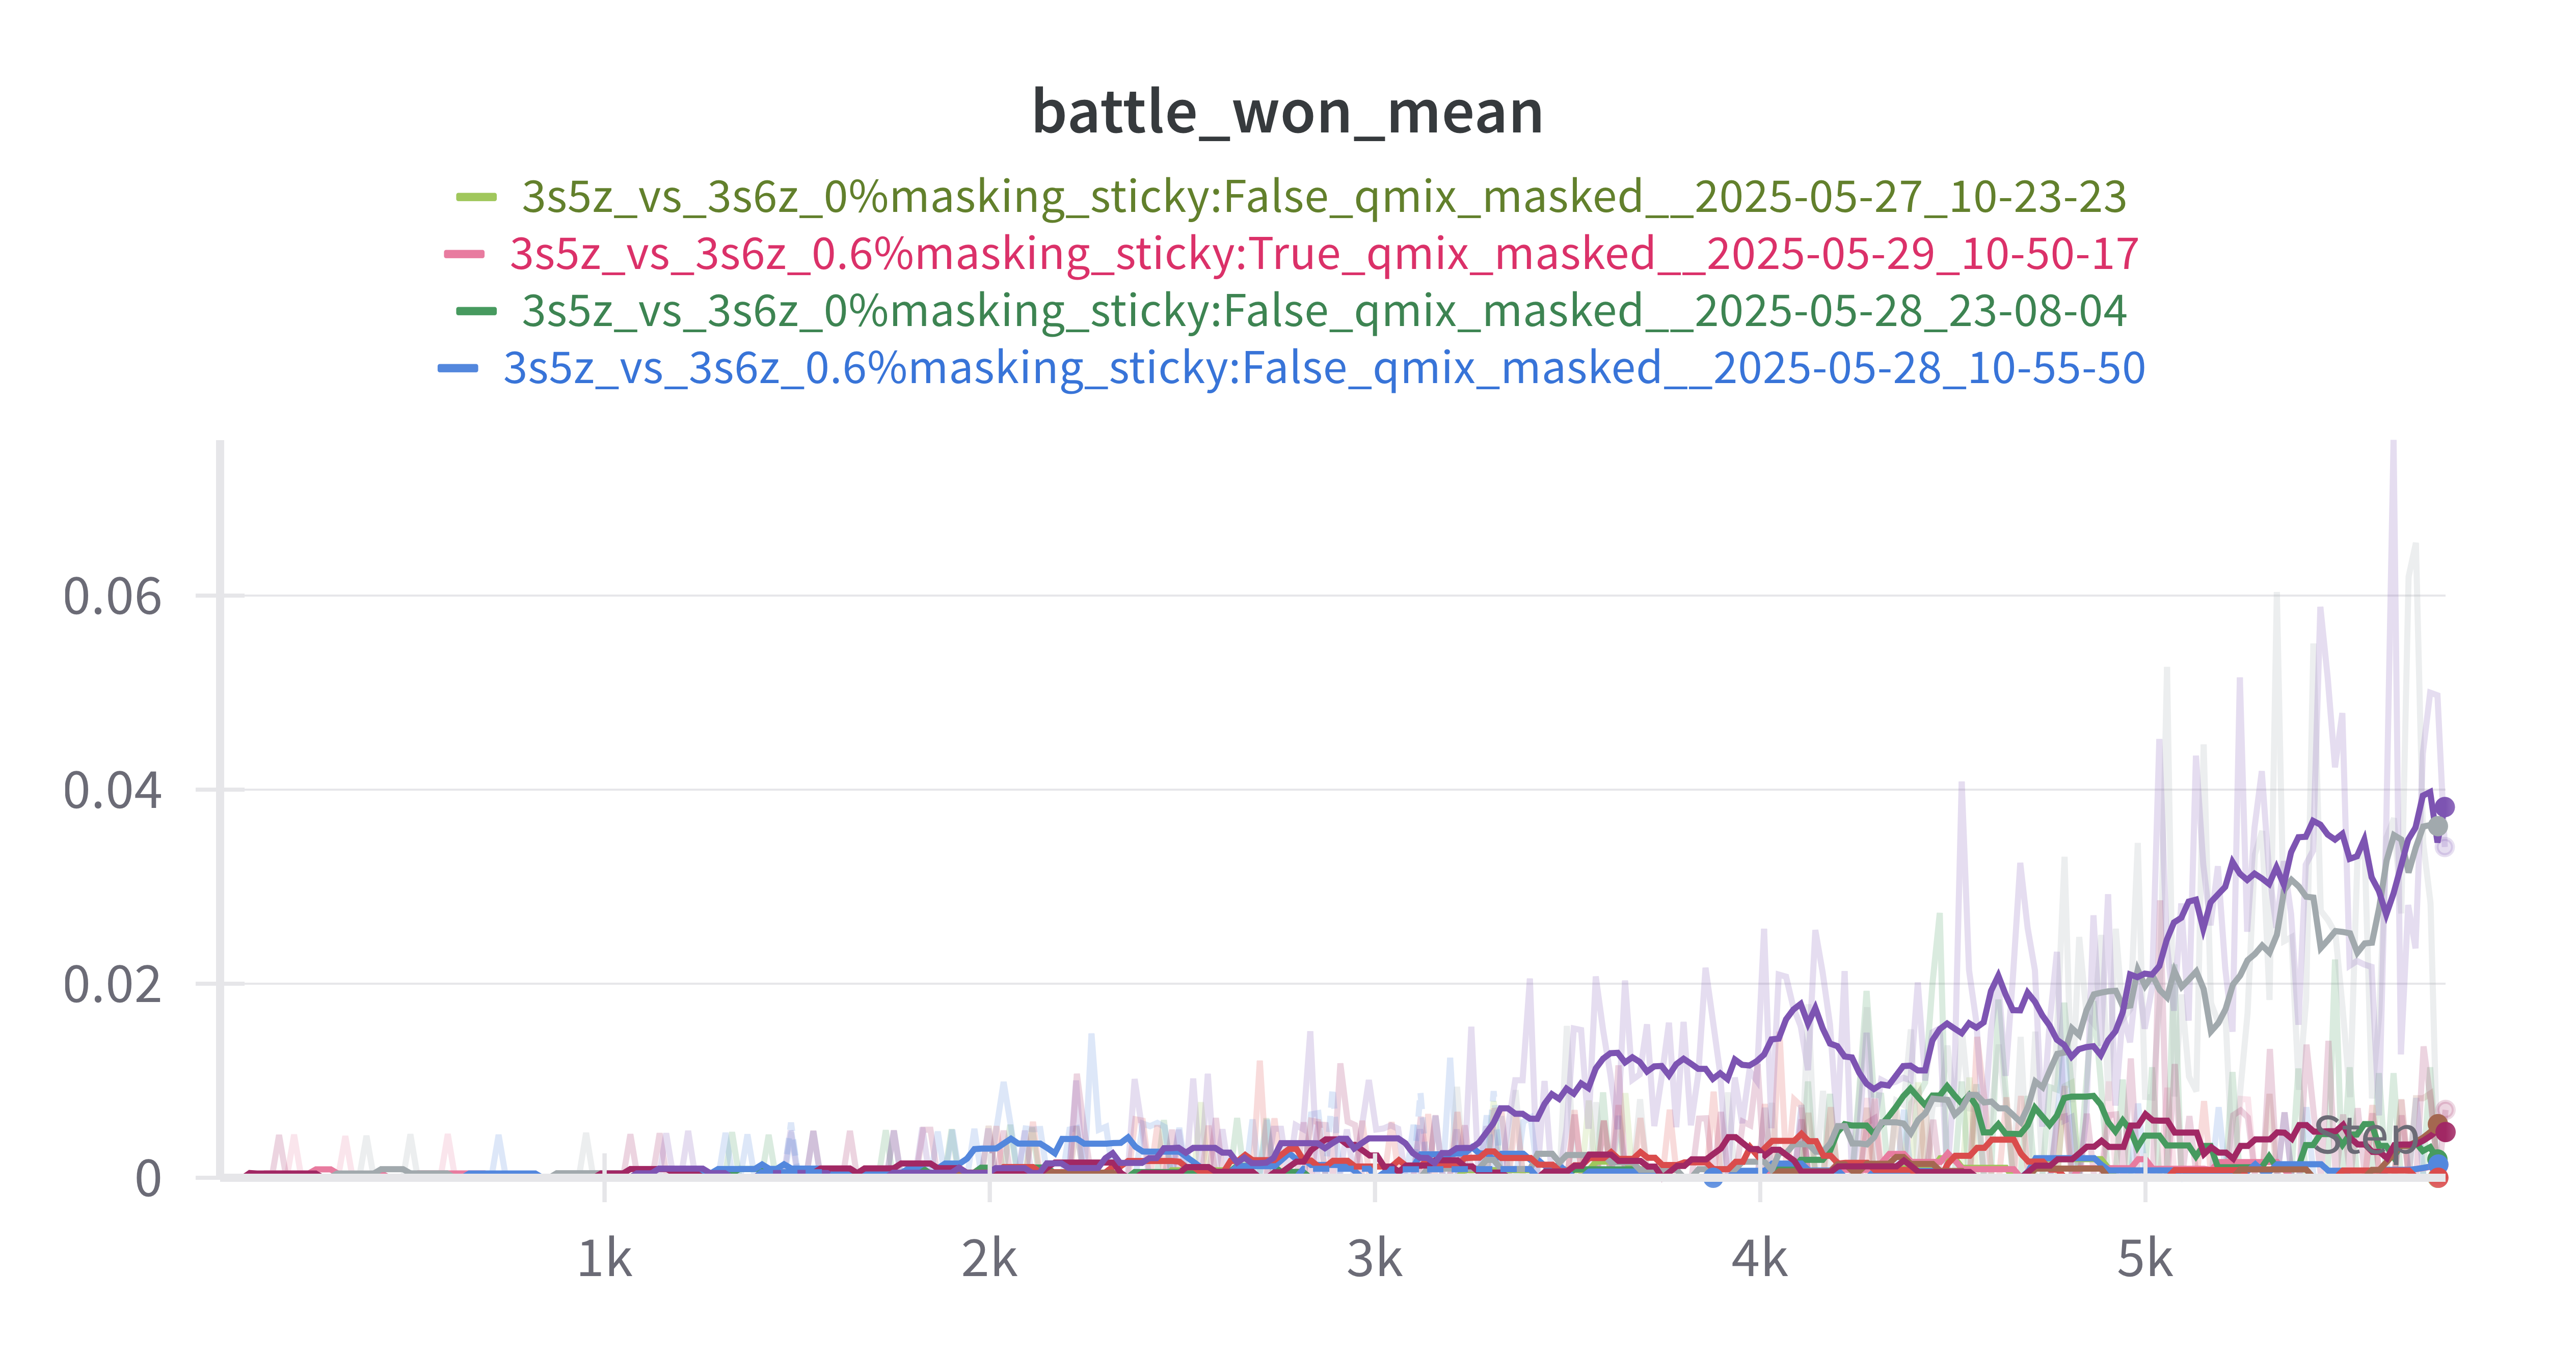
\includegraphics[width=\linewidth]{img/results/3s5z_3s5z.png}
        \caption{\texttt{3s5z\_vs\_3s5z} scenario.}
        \label{fig:3s5z_vs_3s5z}
    \end{subfigure}
    \hfill
    \begin{subfigure}[b]{0.48\textwidth}
        \centering
        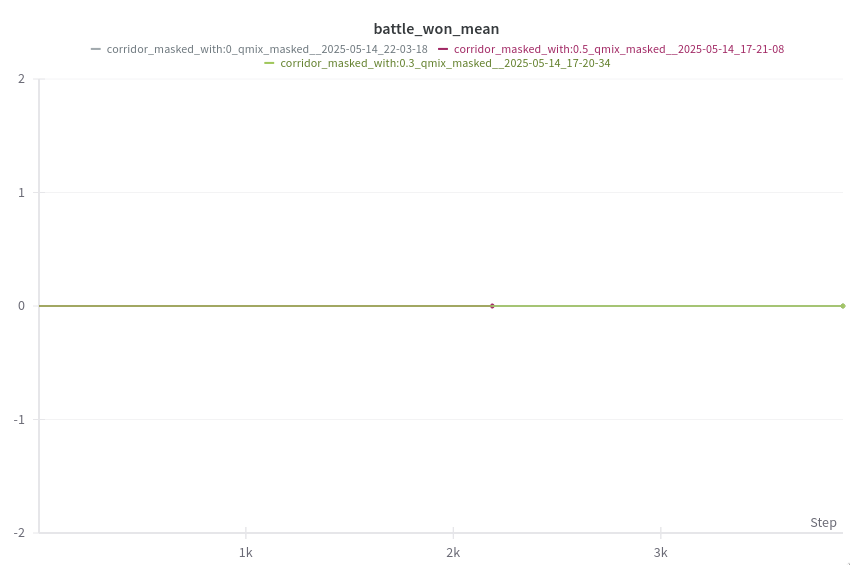
\includegraphics[width=0.95\linewidth]{img/results/corridor.png}
        \caption{\texttt{corridor} scenario.}
        \label{fig:corridor}
    \end{subfigure}
    % \vspace{1em} % Adds vertical space before the final row


    \caption{Performance of baseline QMIX on several hard and super hard SMAC scenarios. The consistently low win rates demonstrate their unsuitability for analyzing the specific impact of masking strategies.}
    \label{fig:hard_scenarios_results}
\end{figure}

Consequently, we selected the \texttt{3s3z} map for our main experiments. This choice is motivated by three factors:
\begin{enumerate}
    \item \textbf{Appropriate Difficulty:} It is a medium-difficulty map where strong coordination is required, but success is achievable.
    \item \textbf{Heterogeneity:} It features two different unit types (Stalkers and Zealots), ensuring our findings are relevant for heterogeneous agent teams.
    \item \textbf{Established Benchmark:} It was a central map used in the original QMIX paper, providing a strong historical baseline.
\end{enumerate}

As shown in Figure~\ref{fig:baseline_2s3z}, our implementation of vanilla QMIX achieves a high and stable win rate on \texttt{3s3z}, establishing a solid baseline against which we can measure the effects of masking.

\begin{figure}[H]
    \centering
    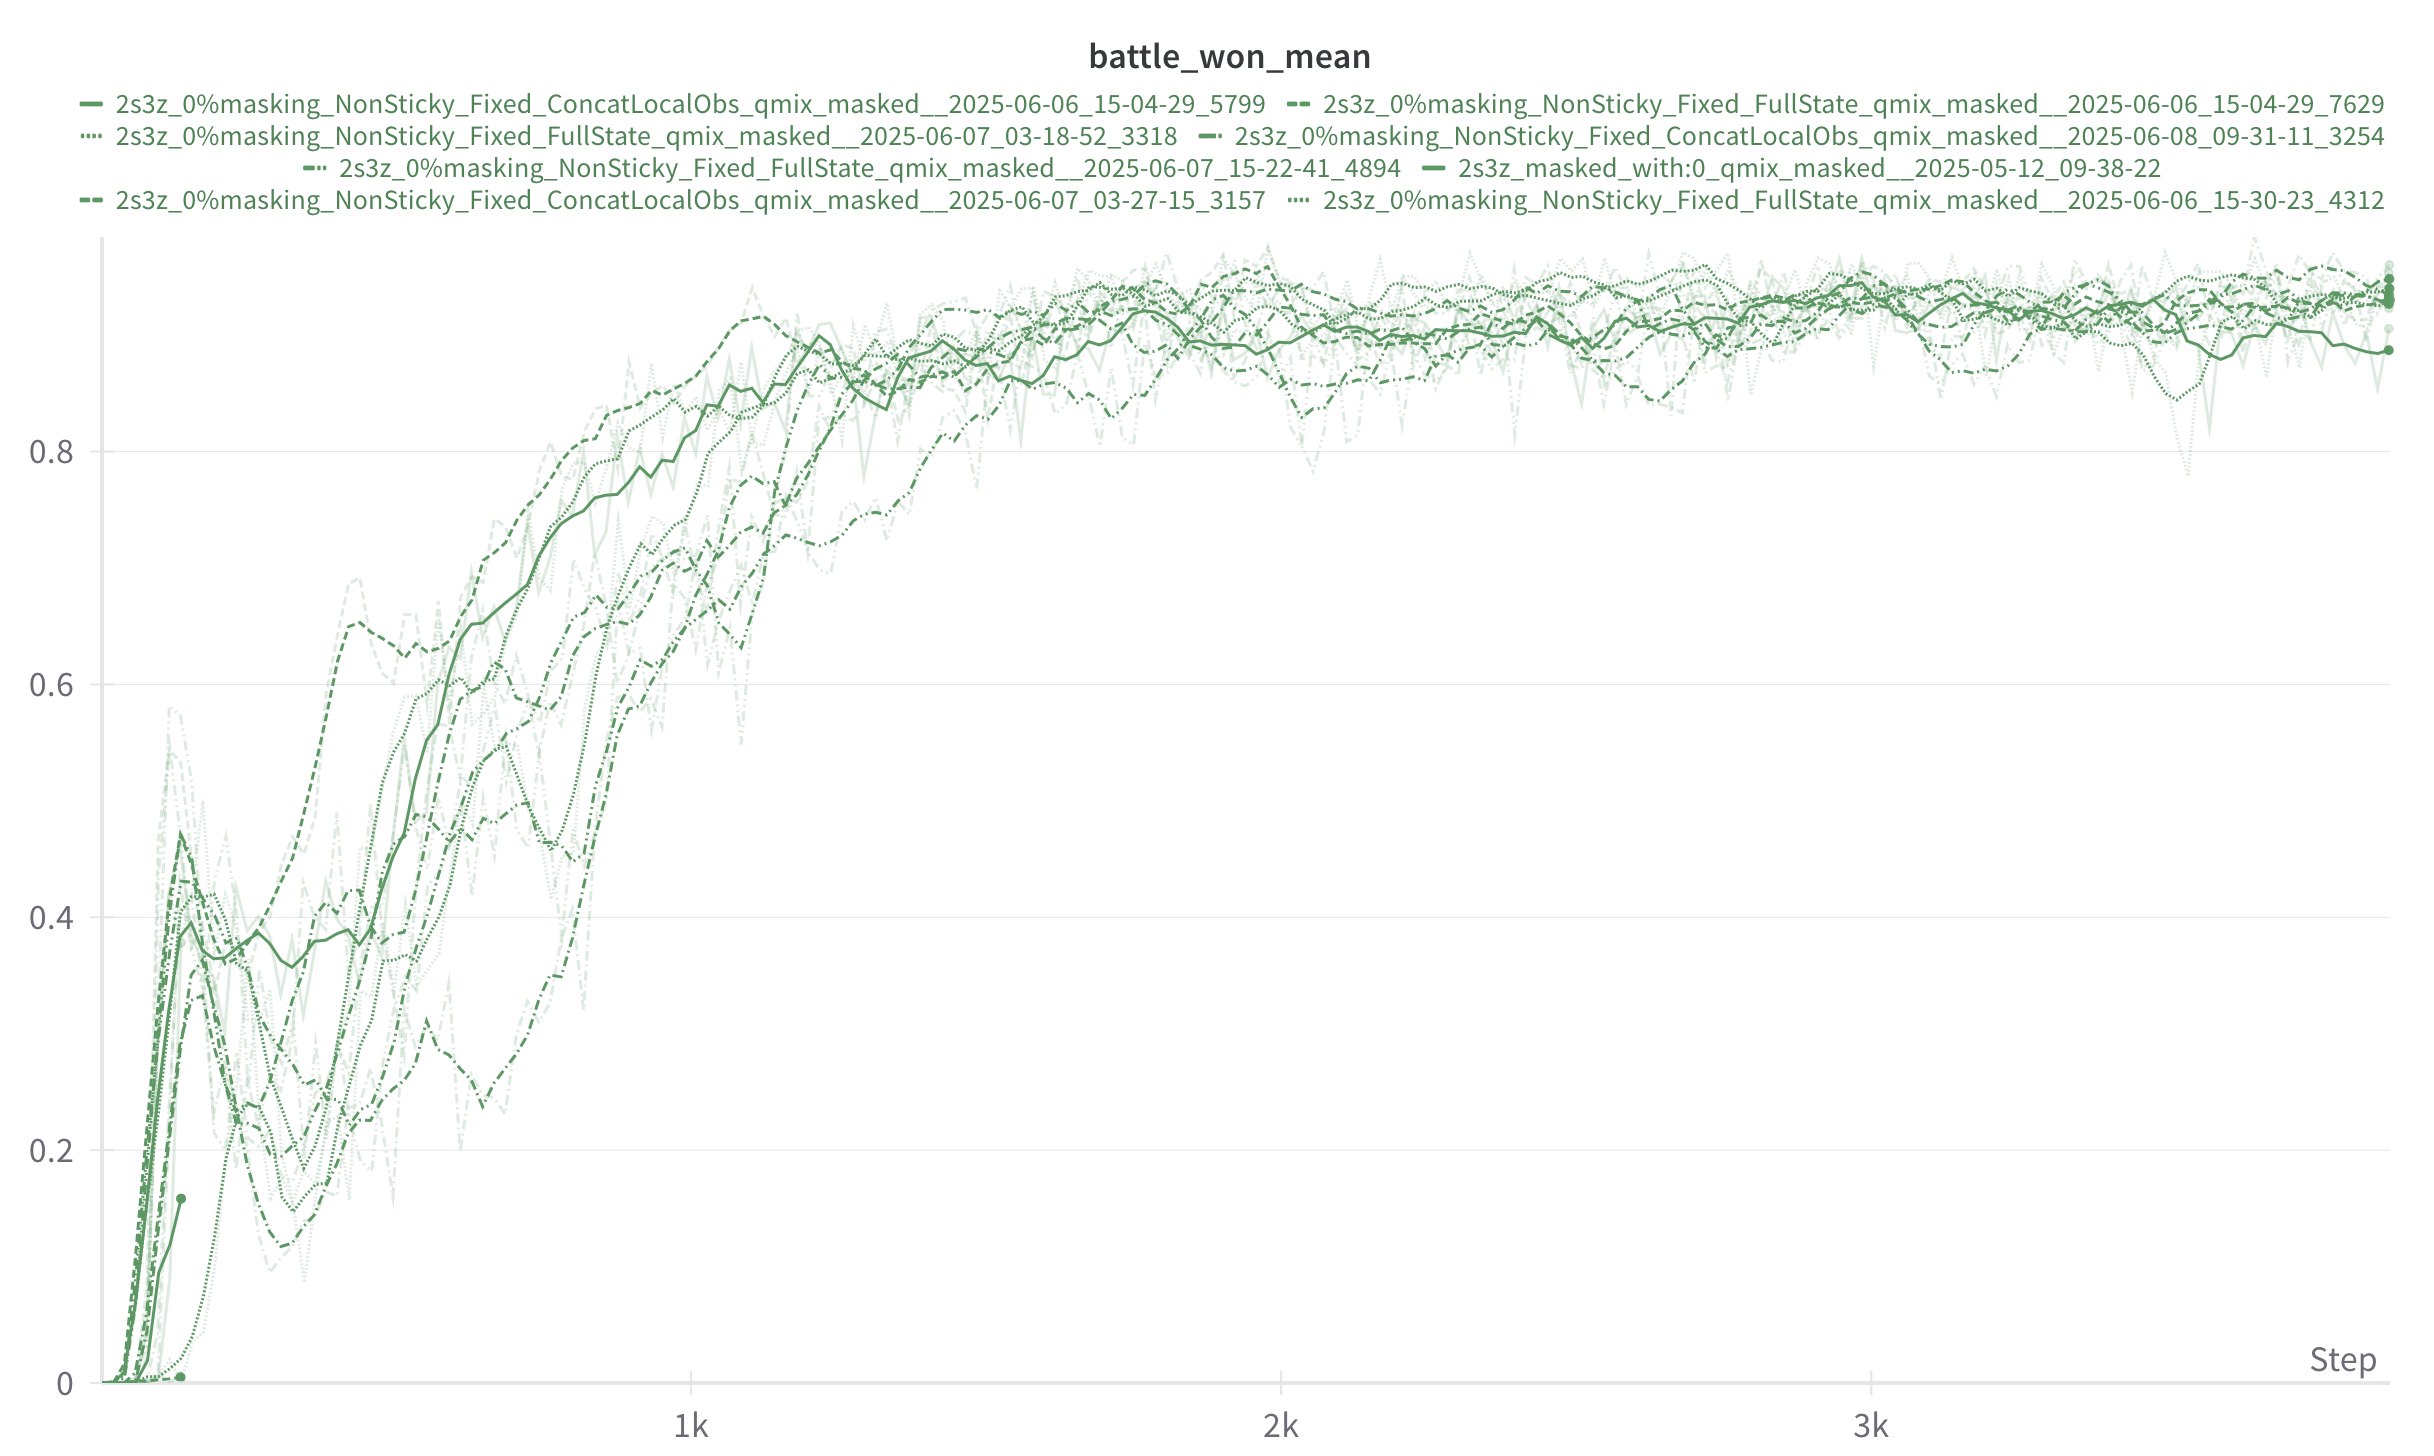
\includegraphics[width=0.6\linewidth]{img/results-analysis/2s3z-baseline.png} % An image showing just the baseline on 2s3z
    \caption{Performance of our baseline vanilla QMIX on the \texttt{3s3z} map, demonstrating a consistent high win rate suitable for comparative analysis.}
    \label{fig:baseline_2s3z}
\end{figure}

\subsection{Evaluating the Impact and Robustness of Random Masking}
With a stable baseline established on \texttt{3s3z}, we proceeded to evaluate the QMIX-Masked variant.

\subsubsection{Effect of Masking Ratio.}
Our first experiment aimed to identify the "breaking point" of the masking strategy. We ran QMIX-Masked with various masking ratios, from 40\% to 70\%. The results, shown in Figure~\ref{fig:masking_ratio_comparison}, reveal a clear trend: performance remains almost identical to the baseline for masking ratios up to 60\%. Beyond this threshold, the win rate begins to drop significantly as critical information is too frequently discarded. This identifies a 60\% masking ratio as the approximate edge of robust performance for this map.

\begin{figure}[H]
    \centering
    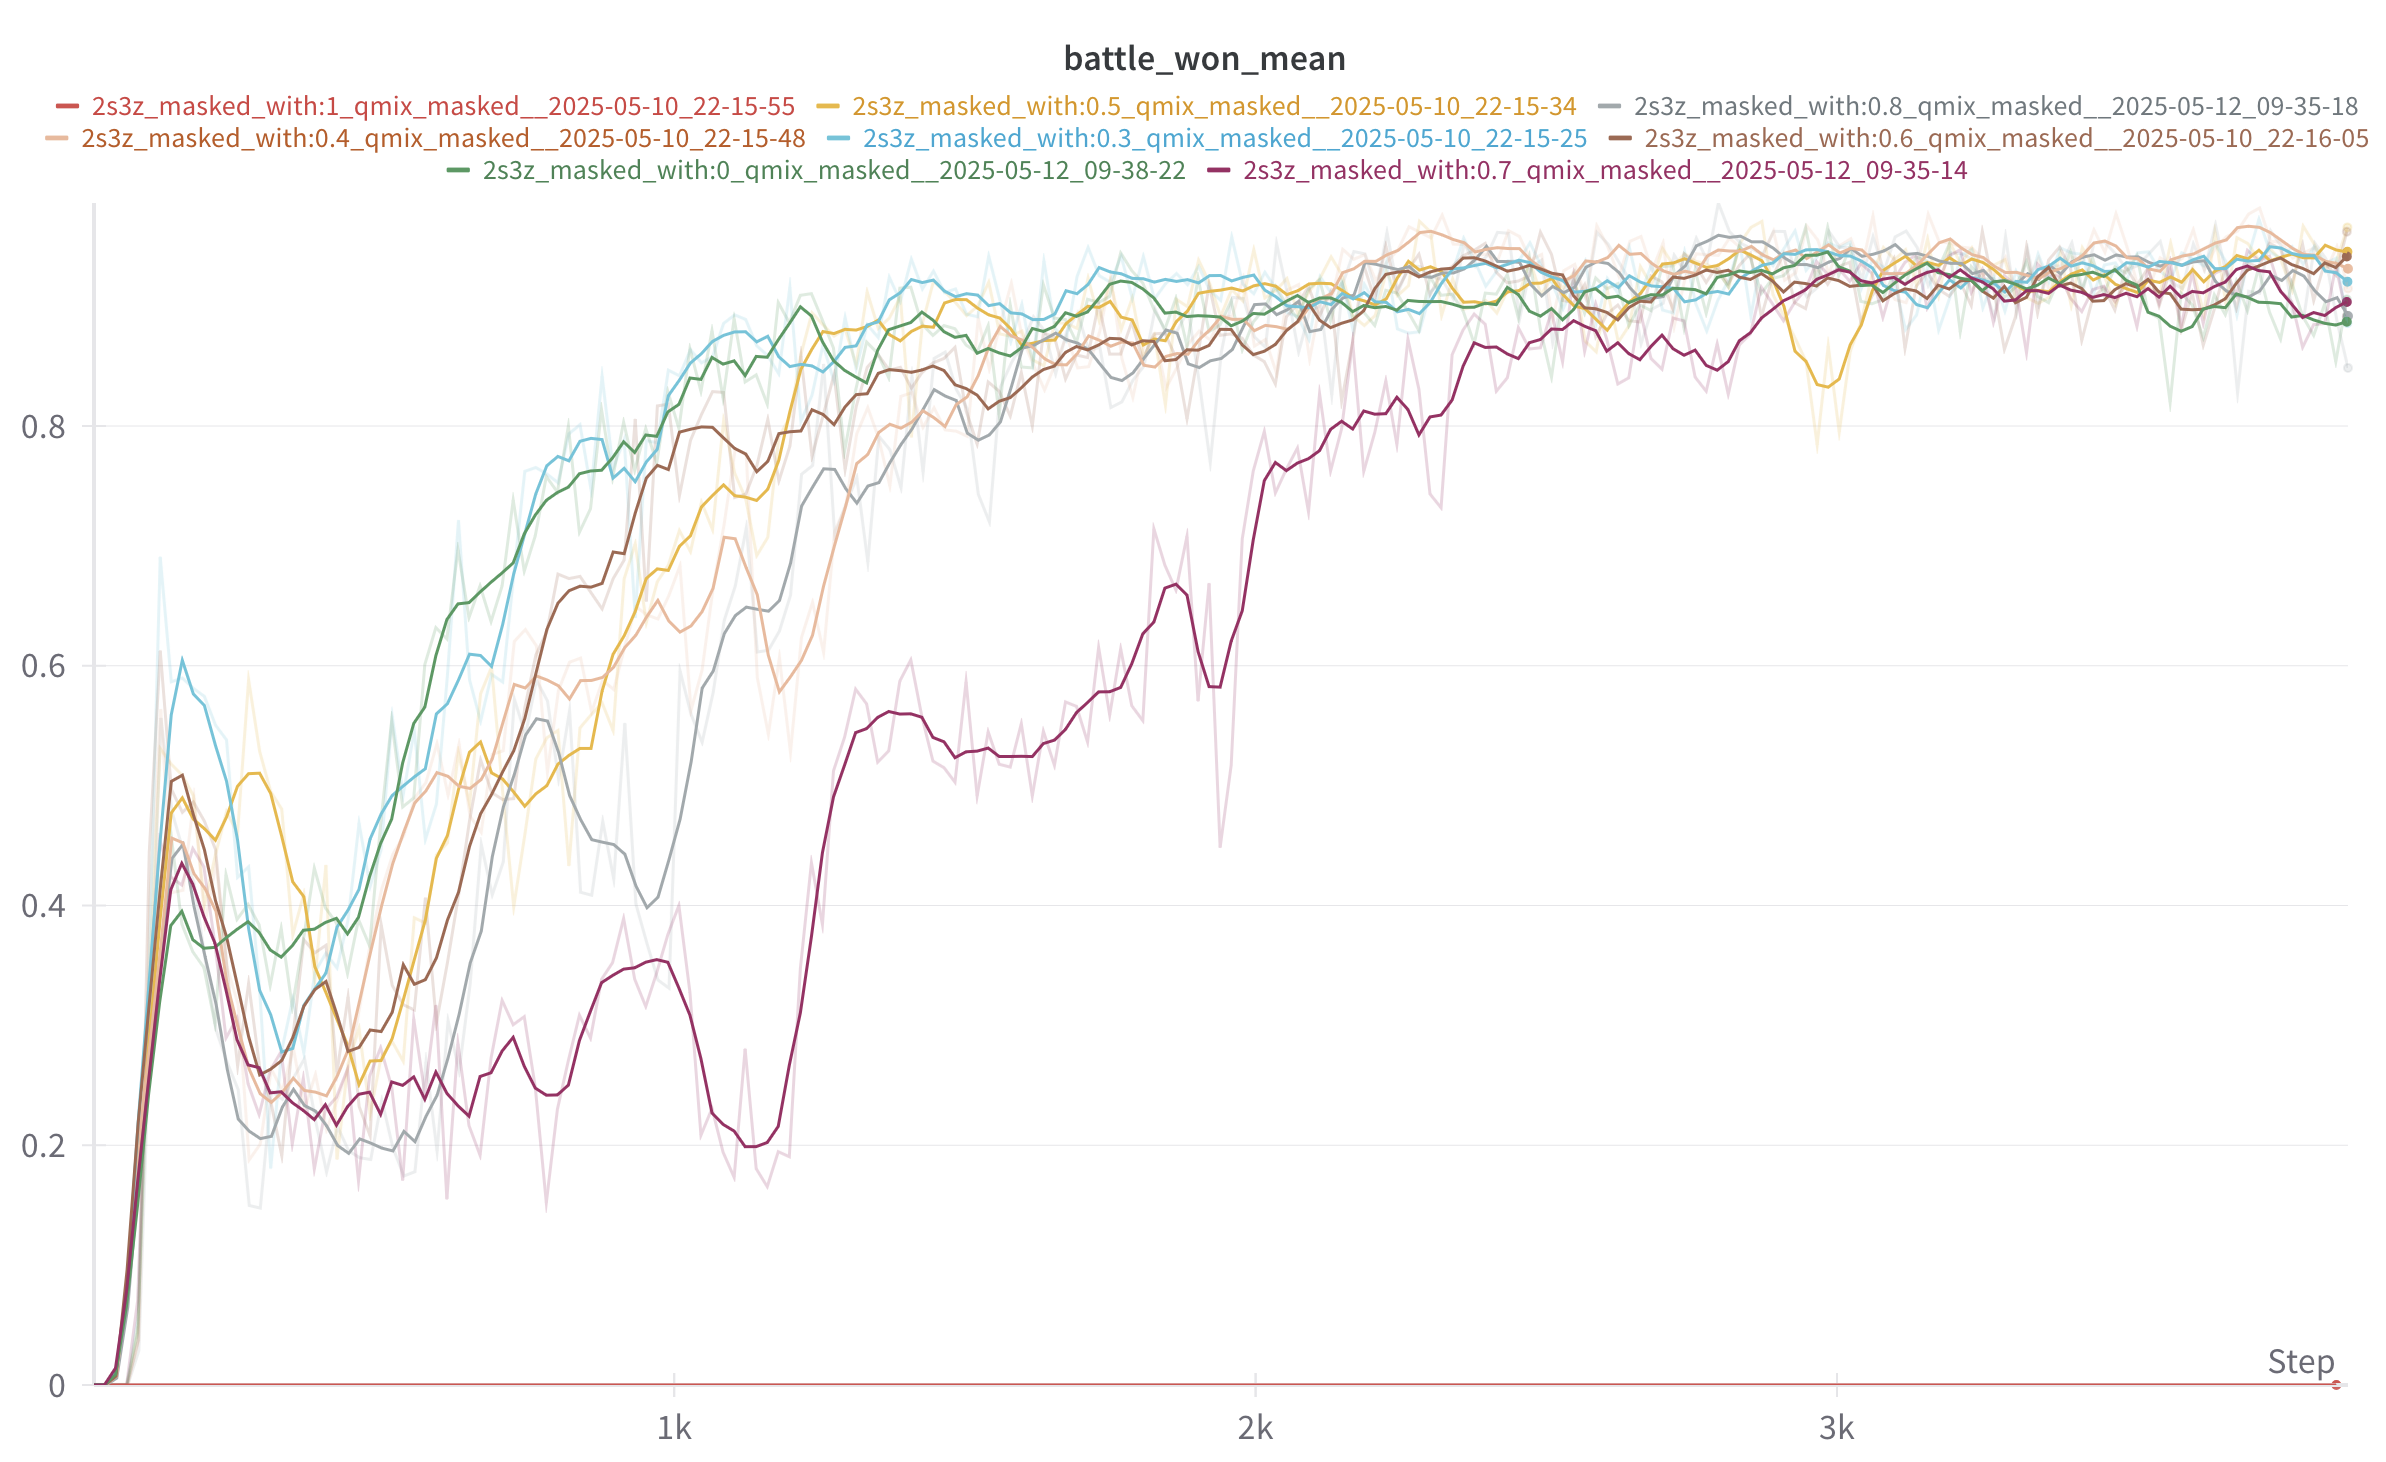
\includegraphics[width=0.7\linewidth]{img/results-analysis/2s3z-multiple-hyperparametrs.png} % An image showing multiple lines for different ratios
    \caption{Comparison of win rates for QMIX-Masked with different masking ratios on \texttt{2s3z}. Performance is stable up to a 60\% ratio before degrading.}
    \label{fig:masking_ratio_comparison}
\end{figure}

\subsubsection{Robustness Analysis.}
We then investigated different types of random masking (standard per-timestep, "sticky" per-episode, and fixed-number). Interestingly, we found no statistically significant performance difference between these strategies. To obtain a more generalizable and statistically robust result for the concept of "random masking," we averaged the results of multiple runs across these strategies using the 60\% ratio.

To directly compare the robustness of the baseline and the 60\% masked variant, we plotted their average performance over multiple seeds with a confidence interval of ±1 standard deviation. As illustrated in Figure~\ref{fig:confidence_comparison}, the learning curves are nearly indistinguishable. The heavily overlapping confidence intervals strongly suggest that, for this scenario, a 60\% random masking introduces no statistically significant performance degradation. This highlights the remarkable robustness of the underlying value decomposition method and suggests that a significant portion of the coordination information may be redundant at any given step.

\begin{figure}[H]
    \centering
    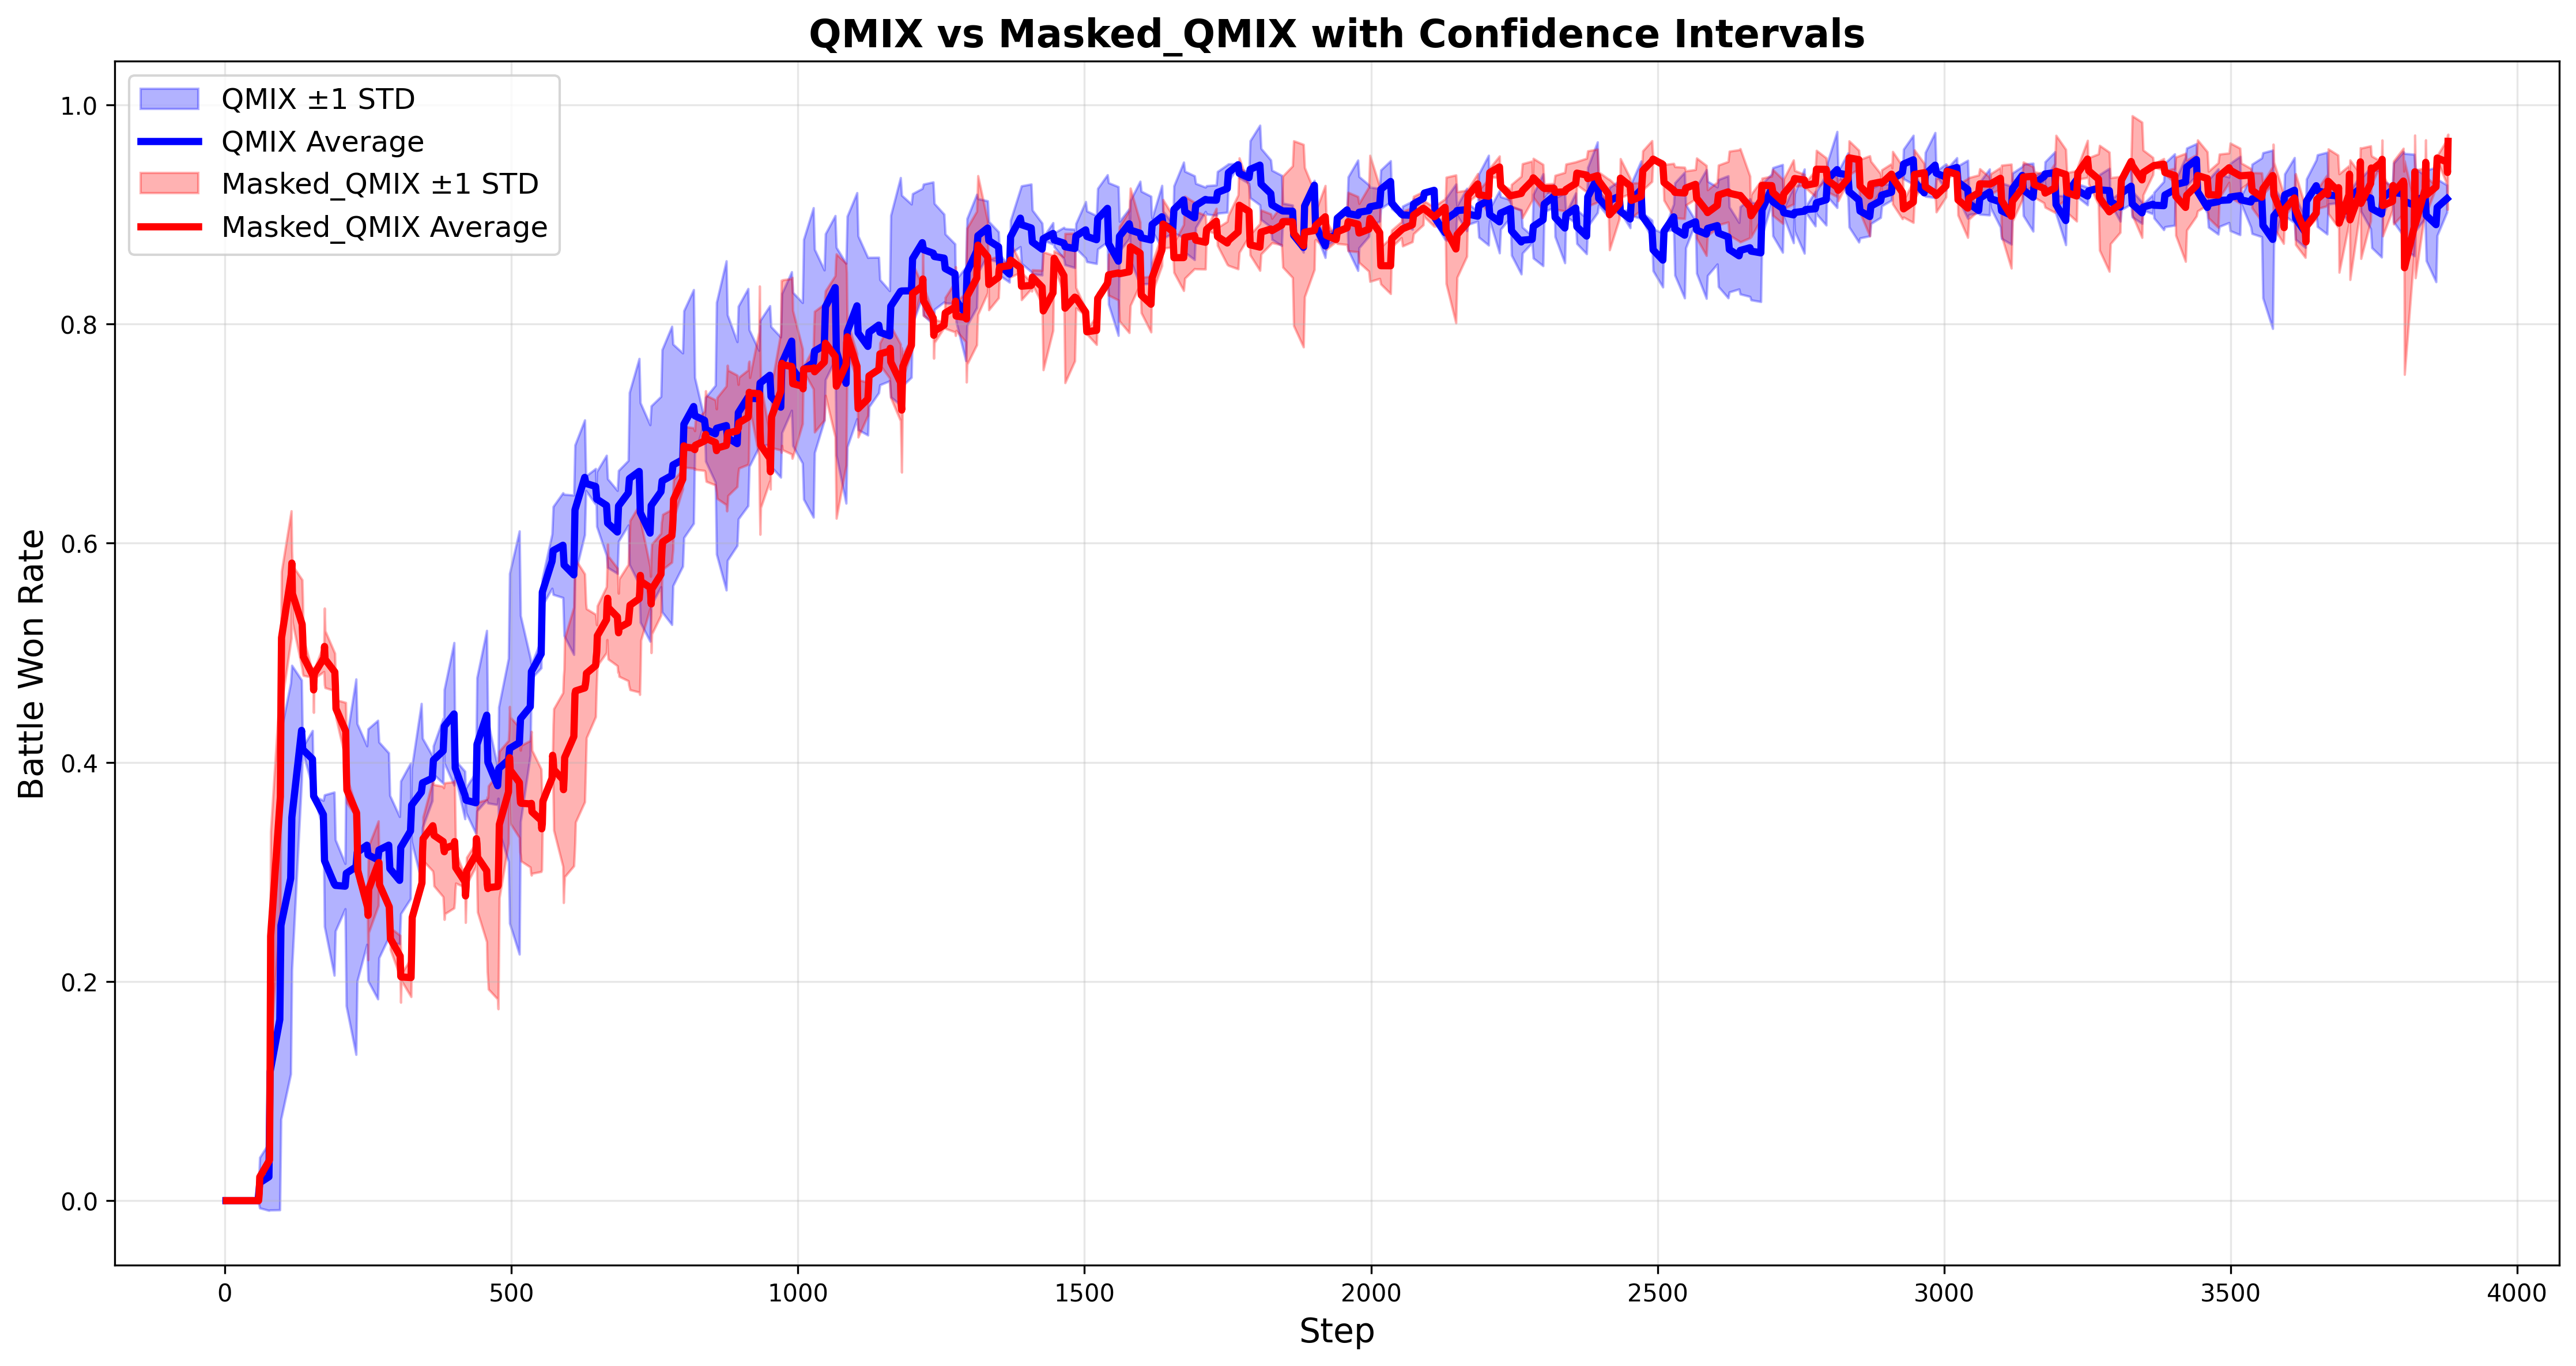
\includegraphics[width=0.7\linewidth]{img/results-analysis/qmix_vs_masked_qmix_with_confidence.png}
    \caption{Averaged performance of baseline QMIX versus QMIX-Masked (60\% ratio) on \texttt{3s3z}. The shaded regions represent ±1 standard deviation over multiple runs. The near-perfect overlap indicates no significant performance loss from masking.}
    \label{fig:confidence_comparison}
\end{figure}


\subsection{Ablation Study on State Conditioning (Ongoing Work)}
In parallel with the masking experiments, we began exploring the impact of the state input used in QMIX’s hypernetwork. Our goal is to determine whether the full global state is necessary for effective mixing or if it can be approximated by simpler, more scalable representations.

Currently, we are investigating three ablation strategies:
\begin{enumerate}
    \item \textbf{No state input:} The hypernetwork is detached from any state input, generating weights purely from its own learned parameters.
    \item \textbf{Local observations only:} The hypernetwork is fed a concatenation of all agents’ local observations instead of the true global state.
    \item \textbf{Unmasked local observations only:} A more aggressive variant where only the local observations of the currently unmasked agents are used as input.
\end{enumerate}

These ablations aim to study how dependent the mixing process is on centralized state information, especially when partial observability and information pruning (via masking) are already part of the training regime. Although conclusive results are not yet available, this line of experimentation is expected to shed light on the feasibility of replacing expensive global state embeddings with cheaper, more scalable alternatives.


\section*{Conclusion}
\addcontentsline{toc}{section}{Conclusion}

This chapter detailed the practical realization and empirical validation of our research into selective coordination. We began by defining a robust and reproducible experimental setup, justifying our choice of the StarCraft Multi-Agent Challenge as the primary testbed. We then articulated the theoretical motivation for our work, highlighting the computational and architectural bottlenecks in the standard QMIX algorithm that arise with an increasing number of agents.

Our core contribution, QMIX-Masked, was introduced as a lightweight variant designed to explore these inefficiencies. Through a carefully structured set of experiments, we demonstrated that random masking is surprisingly robust, with performance on the \texttt{2s\_3z} map remaining statistically indistinguishable from the baseline for masking ratios up to 60\%. This key finding suggests a significant degree of redundancy in the global coordination mechanism of QMIX, opening promising avenues for developing more efficient, intelligent, and scalable multi-agent learning algorithms. The implications of these findings and directions for future work will be discussed in the final chapter of this report.

\end{document}



